% Copyright (C) 2002-2006  Alexei Gilchrist and Paul Cochrane
% 
% This program is free software; you can redistribute it and/or
% modify it under the terms of the GNU General Public License
% as published by the Free Software Foundation; either version 2
% of the License, or (at your option) any later version.
%
% This program is distributed in the hope that it will be useful,
% but WITHOUT ANY WARRANTY; without even the implied warranty of
% MERCHANTABILITY or FITNESS FOR A PARTICULAR PURPOSE.  See the
% GNU General Public License for more details.
%
% You should have received a copy of the GNU General Public License
% along with this program; if not, write to the Free Software
% Foundation, Inc., 59 Temple Place - Suite 330, Boston, MA  02111-1307, USA.

% $Id: /pyscript/local/trunk/doc/manual/libpresentation.tex 4445 2006-06-06T11:33:11.000000Z paultcochrane  $

\chapter{Contributed Optical Components Library}

Alexander Franzen of the Albert-Einstein-Institute in Hannover, Germany has
kindly allowed the use of the objects defined in his Adobe Illustrator 
optical components library in \pyscript.

The components are as follows and are found within the
\texttt{contrib/optics\_components} directory of the \pyscript distribution.
Note that the image of the mode cleaners have been reduced in size to make
the table fit on the page more nicely.

\begin{table}
\begin{tabular}{|c|c|c|c|}
\hline
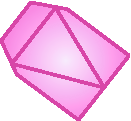
\includegraphics{contrib/optics_components/NPRO} & 
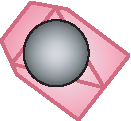
\includegraphics{contrib/optics_components/NPRO_plus_pzt} & 
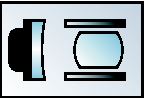
\includegraphics{contrib/optics_components/OPA_SHG_curved_curved} & 

\includegraphics{contrib/optics_components/OPA_SHG_flat_curved}\\
\tiny NPRO & 
\tiny NPRO plus pzt & 
\tiny OPA SHG curved curved & 
\tiny OPA SHG flat curved\\
\hline


\includegraphics{contrib/optics_components/amplifier} & 

\includegraphics{contrib/optics_components/amplitude_phase_modulator1} &
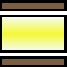
\includegraphics{contrib/optics_components/amplitude_phase_modulator2} & 

\includegraphics{contrib/optics_components/aom}\\
\tiny amplifier & 
\tiny amplitude phase modulator1 &
\tiny amplitude phase modulator2 & 
\tiny aom\\
\hline

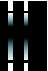
\includegraphics{contrib/optics_components/beam_dump} & 

\includegraphics{contrib/optics_components/beamsplitter_cube} & 

\includegraphics{contrib/optics_components/beamsplitter_plate} & 

\includegraphics{contrib/optics_components/crystal_curved_curved}\\
\tiny beam dump & 
\tiny beamsplitter cube & 
\tiny beamsplitter plate & 
\tiny crystal curved curved\\
\hline


\includegraphics{contrib/optics_components/crystal_flat_curved} & 

\includegraphics{contrib/optics_components/crystal_flat_flat} & 
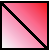
\includegraphics{contrib/optics_components/dichroic_beamsplitter_cube} &

\includegraphics{contrib/optics_components/dichroic_mirror1}\\
\tiny crystal flat curved & 
\tiny crystal flat flat & 
\tiny dichroic beamsplitter cube &
\tiny dichroic mirror1\\
\hline


\includegraphics{contrib/optics_components/dichroic_mirror2} & 
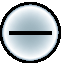
\includegraphics{contrib/optics_components/difference} &

\includegraphics{contrib/optics_components/faraday_rotator} &

\includegraphics{contrib/optics_components/flip_mirror}\\
\tiny dichroic mirror2 & 
\tiny difference &
\tiny faraday rotator &
\tiny flip mirror\\
\hline


\includegraphics{contrib/optics_components/frequency_generator1} & 

\includegraphics{contrib/optics_components/frequency_generator2} & 

\includegraphics{contrib/optics_components/grating} &

\includegraphics{contrib/optics_components/highpass_filter}\\
\tiny frequency generator1 & 
\tiny frequency generator2 & 
\tiny grating &
\tiny highpass filter\\
\hline


\includegraphics{contrib/optics_components/hv_amplifier1} & 

\includegraphics{contrib/optics_components/hv_amplifier2} & 

\includegraphics{contrib/optics_components/laser1} &
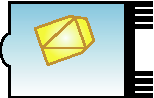
\includegraphics{contrib/optics_components/laser2}\\
\tiny hv amplifier1 & 
\tiny hv amplifier2 & 
\tiny laser1 &
\tiny laser2\\
\hline


\includegraphics{contrib/optics_components/laser_diode} & 

\includegraphics{contrib/optics_components/lens_concave_concave} &

\includegraphics{contrib/optics_components/lens_convex_convex} &

\includegraphics{contrib/optics_components/lens_flat_convex}\\
\tiny laser diode & 
\tiny lens concave concave &
\tiny lens convex convex &
\tiny lens flat convex\\
\hline


\includegraphics{contrib/optics_components/lowpass_filter} & 

\includegraphics{contrib/optics_components/mirror_curved} & 

\includegraphics{contrib/optics_components/mirror_curved_with_pzt} &

\includegraphics{contrib/optics_components/mirror_flat}\\
\tiny lowpass filter & 
\tiny mirror curved & 
\tiny mirror curved with pzt &
\tiny mirror flat\\
\hline


\includegraphics{contrib/optics_components/mirror_with_pzt} & 

\includegraphics{contrib/optics_components/mixer} & 
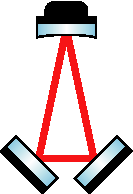
\includegraphics[height=1cm]{contrib/optics_components/mode_cleaner_with_pzt} &
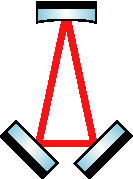
\includegraphics[height=1cm]{contrib/optics_components/mode_cleaner_without_pzt}\\
\tiny mirror with pzt & 
\tiny mixer & 
\tiny mode cleaner with pzt &
\tiny mode cleaner without pzt\\
\hline


\includegraphics{contrib/optics_components/optical_diode1} & 

\includegraphics{contrib/optics_components/optical_diode2} &
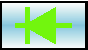
\includegraphics{contrib/optics_components/optical_diode_green} &

\includegraphics{contrib/optics_components/photodetector1}\\
\tiny optical diode1 & 
\tiny optical diode2 &
\tiny optical diode green &
\tiny photodetector1\\
\hline


\includegraphics{contrib/optics_components/photodetector2} & 

\includegraphics{contrib/optics_components/photodetector3} & 

\includegraphics{contrib/optics_components/photodetector4} &

\includegraphics{contrib/optics_components/servo1}\\
\tiny photodetector2 & 
\tiny photodetector3 & 
\tiny photodetector4 &
\tiny servo1\\
\hline


\includegraphics{contrib/optics_components/servo2} & 
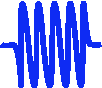
\includegraphics{contrib/optics_components/single_mode_fibre} & 
\includegraphics{contrib/optics_components/spectrum_analyser} &
\includegraphics{contrib/optics_components/sum}\\
\tiny servo2 & 
\tiny single mode fibre & 
\tiny spectrum analyser &
\tiny sum\\
\hline

\includegraphics{contrib/optics_components/sum_difference} & 
\includegraphics{contrib/optics_components/waveplate1} &
\includegraphics{contrib/optics_components/waveplate2} &
\includegraphics{contrib/optics_components/waveplate3}\\
\tiny sum difference & 
\tiny waveplate1 &
\tiny waveplate2 &
\tiny waveplate3\\
\hline
\end{tabular}
\caption{Contributed optical component library}
\end{table}

